SE and opinion mining is the field of study that analyzes people's opinions, sentiments, evaluations, attitudes, and emotions from written language.\cite{liu2012sentiment} It's also known as emotion AI or opinion mining. The main and basic task of this field is to correctly classify the polarity of a particular text and evaluate whether is it positive, negative or in some cases neutral. It can be used in almost any situation where data need to be analysed for its sentiment aspect, what means the application options are almost endless.  for example product reviews, online discussions or social media content.

SE is in demand mostly because of its efficiency. Tens of thousands of documents can be analysed within seconds and despite results are not always as exact as human workers would produce, the efficiency boost is often too big not to take advantage of it.

SE can be divided into several steps:
\begin{enumerate}
  \item \textbf{Data collection} - involves all the substeps required to gather user-generated content from any source. Surveys, blogs, various forums and social media. These all contains huge amount of real people from real world with real experiences. These data are always expressed completely different - using slang, shortcuts, internet language or generally just being used in different context.
  \item \textbf{Data preprocessing} - this step represents cleaning the data. Data preprocessing can often have a significant impact on generalization performance of a supervised ML algorithms \cite{kotsiantis2006data} and if there is much irrelevant information and data are unreliable, then knowledge discovery during the training phase is more difficult. It removes irrelevant content which could potentially lead to bad and incorrect results. This is a very delicate step because it manipulates the raw data and if not done correctly, it can easily change results.
  \item \textbf{Sentiment detection} - this step basically stands for training of the classifier. Subjective feelings and expressions are highlighted, emphasized and retained while objective information like facts are discarded and ignored. 
  \item \textbf{Sentiment classification} - subjective expressions are classified.
    \item \textbf{Output interpretation} - graphical presentation of obtained results. Time and sentiment can be analyzed to construct various charts, graphs, timelines and many other metrices.
\end{enumerate}

\section{History}
Interest in opinion of other individuals is probably as old as the communication itself. There is evidence that already in ancient Greece, generals were trying to detect dissent among their subordinates using various "primitive" approaches \cite{richmond1998spies}. Another approach to measure and evaluate a public opinion coming from ancient Greece and used to these date is voting. In the first decades of twentieth century, efforts in capturing public opinion started utilize questionaires and in 1937, first scientific journal on public opinion was founded. 

In the last 10 years, SE and ML in general experienced a big boom. According to data collected by Mantyla, Graziotin and Kuutila \cite{mantyla2018evolution}, nearly 7000 papers about sentiment analysis have already been written and not surprisingly, 99\% of them were published after 2004 - making sentiment analysis one of the fastest growing research areas. The increasing interest about this area as published by Mantyla, Graziotin and Kuutila \cite{mantyla2018evolution} can be seen in the graph \ref{fig:papersCountHistory}.

\begin{figure}[H]%
    \centering
	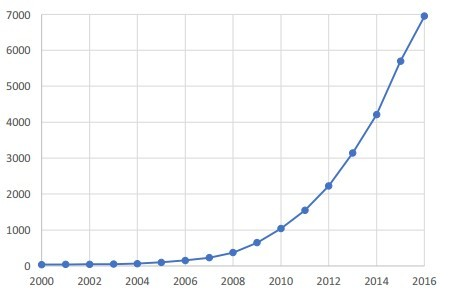
\includegraphics[width=8cm]{papersCountHistory.jpg}
    \caption{Cumulative count of papers about sentiment analysis}%
    \label{fig:papersCountHistory}%
\end{figure}



\section{Training datasets} \label{sec:trainingDatasets}
One of the main building blocks of any correctly and accurately functioning ML projects is a training phase. It can actually be seen as a base for the whole project. One can have the best fine-tuned optimized classifier, but if the training data he used do not fit the domain where the classifier is intended to be used, results of the classifier can be (surprisingly) bad. It's the same as house and its base. If the base is not done correctly, however cool architectural solution have other storeys used, house is still going to fall in the next big storm.

That's why choosing a sufficient and fitting dataset to train my classifiers was a very important task. The datasets I've considered were:
\begin{itemize}
  \item \textbf{Dataset140}\footnote{http://cs.stanford.edu/people/alecmgo/trainingandtestdata.zip} - it is currently the biggest dataset with tweets labeled by their sentiment. What is interesting and makes the dataset special is that opposed to other datasets being manually annotated by humans, this one was created by a program. It contains 1.6 million tweets with their polarity score (0 = negative, 2 = neutral, 4 = positive), tweet id, date of tweet publication, author of the tweet and the text of the tweet. More about how this dataset was created can be found in Go et al. paper \cite{go2009twitter}
  \item \textbf{Movie review data}\footnote{http://www.cs.cornell.edu/people/pabo/movie-review-data/} - Thousand positive and thousand negative labeled movie reviews. This dataset was introduced in Pang/Lee ACL 2004 \cite{pang2004sentimental}
  \item \textbf{Hu-Liu lexicon}\footnote{https://github.com/woodrad/Twitter-Sentiment-Mining/tree/master/Hu\%20and\%20Liu\%20Sentiment\%20Lexicon} - plain list of 6800 common English words labeled as positive and negative
  \item \textbf{Warriner et al lexicon}\footnote{http://crr.ugent.be/archives/1003} - This list of words was collected with Amazon Mechanical Turk. Three components of emotions are distinguished: valence (the pleasantness of a stimulus), arousal (the intensity of emotion provoked by a stimulus), and dominance (the degree of control exerted by a stimulus) \cite{warriner2013norms}. Warriner and Kuperman extended ANEW norms collected by Bradley and Lang from 1034 words to 13,915 words (lemmas).
  \item \textbf{Stack overflow dataset}\footnote{https://sentiment-se.github.io/replication.zip} - Later into the thesis I've decided to test dataset of 1500 manually labeled Stack overflow sentences created by Bin Lin et al. in their late paper on negative results in SA called "How far can we go".
    \item \textbf{My own cryptocurrency tweets dataset} - As already said before, performance of the classifier depends on how close the training data are to the real use-case data. That's why I considered and even started to create my own dataset targeting specifically only cryptocurrency tweets, which I've intended to analyze as well.
\end{itemize}

Big surprise here was the lack of any bigger Reddit dataset.

\section{Language processing tools} \label{sec:languageProcessingTools}
From the very beginning, I knew I wanted to use Python. I had some slight background knowledge in ML from online courses and most of them were done in Python. Therefore while searching and deciding which library should I use, I've always given a slight edge to the Python options. I've considered (and tested) these:
\begin{itemize}
\item \textbf{NLTK} - probably the best-known Python module for NLP. It provides easy-to-use interfaces for more than 50 corpora and lexical resources. It also offeres a rich palette of processing libraries for classification, tokenization, stemming, tagging, parsing, and semantic reasoning.
\item \textbf{Textblob: Simplified Text Processing} - as a name says, Textblob provides easy processing and is actually built on top of NLTK. It provides a simple API for diving into common natural language processing tasks such as part-of-speech tagging, noun phrase extraction, sentiment analysis (Naive Bayes, Decision Tree), classification, translation and more.
\item \textbf{Scikit-learn} - Python module for general ML, data mining and data analysis. It is built on NumPy, SciPy and matplotlib modules.
\end{itemize}

Also, sentiment analysis is just one part of the task. To evaluate the data and find pattern, basic data science algorithms will be needed. With data science, R is very often listed as a default choice. Therefore were the results of google trends query shown in Figure  pretty surprising. This definitely helped my decision with sticking to Python.

\begin{figure}[H]%
    \centering
	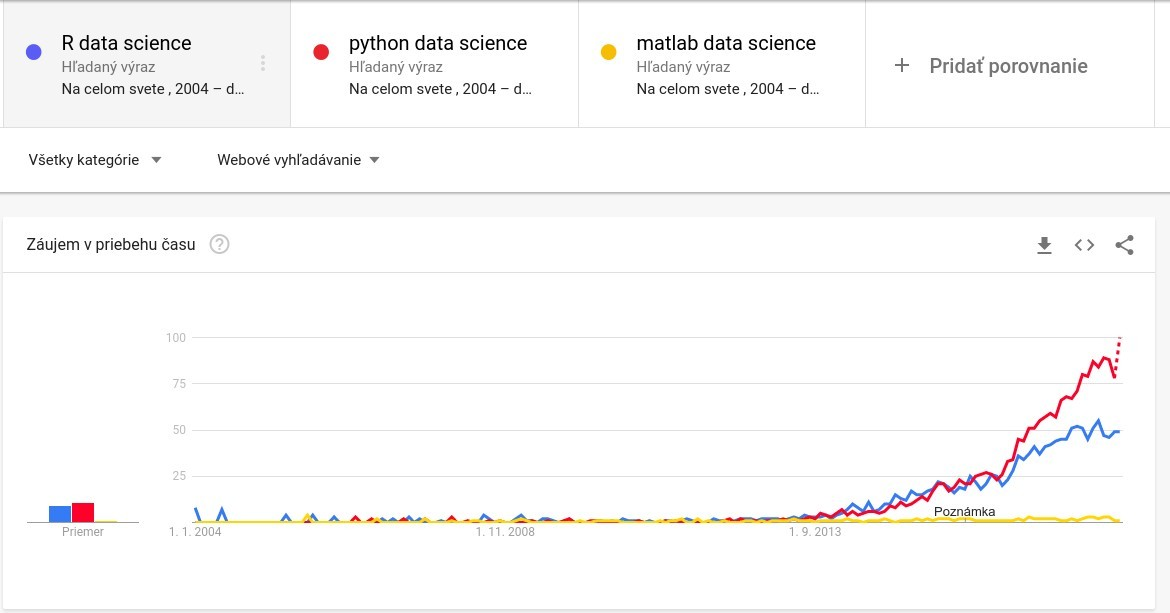
\includegraphics[width=10cm]{PythonMatlabR.jpg}
    \caption{Google trend of searches regarding data science with various programming languages}%
    \label{fig:PythonMatlabR}%
\end{figure}


\section{Performance metrics}
\paragraph{Terminology} Before diving into talk about the metrics, there are 4 crucial terms which need to be explained:
\begin{itemize}
\item \textbf{Tue Positives (TP)} - instances correctly labeled as positive
\item \textbf{True Negatives (TN)}- instances correctly labeled as negative
\item \textbf{False Positives (FP)} - instances incorrectly labeled as positive
\item \textbf{False Negatives (FN)}- instances incorrectly labeled as negative
\end{itemize}


The metrics that you choose to evaluate your machine learning algorithms are very important and not all are suitable for every situation. Choice of metrics influences how the performance of machine learning algorithms is measured and choosing a wrong evaluation metric for particular use could potentially lead towards eliminating the best performing algorithm in favour of the worse one.
Here are some of the most often used metrics used to evaluate classification algorithms. It's also useful to choose the metric before doing the analysis, so you won't get distracted by already having the results in case of doing the decision later.

\begin{itemize}
\item \textbf{Classification accuracy} - this is the most intuitive and common evaluation metric for classification problems but it is also the most misused one. It is really only suitable when there are an equal number of observations in each class (which is rarely the case) and that all predictions and prediction errors are equally important, which is often not the case. In case of imbalanced dataset with 9\% of instances in one class and only 10\% in the other, predicting every instance as a majority class without even considering its features would lead to high accuracy of 90\%. This is called \textbf{accuracy paradox.}
\[ Accuracy = \frac{TP + TN}{TP + TN + FP + FN}\]
\item \textbf{Confusion matrix} - clean and unambiguous way to present the prediction results of a classifier. If the classification is binary (there are only 2 classes), this matrix has 2 rows and 2 columns - therefore altogether 4 cells which are filled with true/false positives/negatives count. Such scenario is demonstrated in table \ref{table:Confusion_matrix_general}. Although the confusion matrix shows all of the information about the classifier's performance, more meaningful measures can be extracted from it to illustrate certain performance criteria.\cite{bradley1997use}. 
\begin{table}[H]
{
\centering
\begin{tabular}{ |p{4cm}|p{4cm}|p{4cm}|  }
 \hline
 \multicolumn{3}{|c|}{Confusion matrix} \\
 \hline
  & Predicted positive & Predicted negative\\
 \hline
 Real positive   & TP    &FN\\ \hline
 Real negative &   FP  & TN\\ \hline
\end{tabular}
}
\caption{Confusion matrix}
\label{table:Confusion_matrix_general}
\end{table}

\item \textbf{Precision} - Precision can be seen as a representation of a classifiers exactness. A low precision can also indicate a large number of False Positives. If the precision is high, it says that there's a high probability of positive label being True Positive. It cannot be tricked but it also hides a lot.
\[ Precision = \frac{TP}{TP + FP}\]
\item \textbf{Recall} - also called \textit{sensitivity} or the \textit{True Positive Rate}, it is a number of True Positives divided by the number of True Positives and the number of False Negatives. In other words, it is a ratio of how many of all positive instances have been identified. Recall can be tricked (labeling all as majority class) but if used next to precision, it gives extra information
\[ Recall = \frac{TP}{TP + FN}\]
\item \textbf{F measure} - as already mentioned, precision hides some facts and recall can be tricked. To give the full story, they need to be used together. That's what F measure is for.
\[ F = 2 * \frac{precision * recall}{precision + recall}\]
\end{itemize}Nice example to demonstrate difference between precision and recall is the concept of Indian Jurisprudence, where "100 culprits may let go free but no innocent should be punished". If we let go so many culprits in order to ensure no innocent is punished, recall will be pretty low, but precision very high.

\section{Classifier evaluation}
\label{sec:classifierEvaluation}
All the testing has been done on the testing data supplied within Sentiment140.

\paragraph{Textblob:}
As a first option, I executed the analysis with Python TextBlob. Sentiment polarity returned by Textblob is a float value in range from -1 to 1 where positive values stand for positive sentiment and negative values for negative sentiment. Bigger the absolute value of output, stronger the sentiment is. This solution didn't need any training data or labeled dataset of positive and negative words because it already comes with trained classifiers. This alone was the reason why I felt that it might not be the best performing classifier. Because returned scores are floats and Sentiment140 tweets are labeled with just positive/negative, I had to execute a small transformation of the output. Interesting point in the transformation was handling of the zero(neutral) score. In the following table \ref{table:TextblobNeutralTweetResolvingResults} are shown several considered transformation options and from them resulting accuracy of the model. 

\begin{table}[H]
\centering
\begin{tabular}{ |p{3cm}||p{3cm}|}
 \hline
\textbf{ Score = 0 }& \textbf{Accuracy}\\
 \hline
 Label as positive   & 0.608944\\ \hline
 Label as negative & 0.622649\\ \hline
 Ignore & 0.679612\\ \hline 
\end{tabular}
\caption{Textblob accuracy with various handling of neutral tweets}
\label{table:TextblobNeutralTweetResolvingResults}
\end{table}

Obviously, none of these primitive approaches is the correct one. How to handle neutral class in sentiment analysis is still pretty open question and some possible approaches will be discussed later.


As mentioned earlier, accuracy is not the best metric to evaluate classifiers on, but with such low values, it is apparent that Textblob isn't performing very well. There might be several reasons for this:
\begin{itemize}
\item Tweets are in general difficult to analyze because they are limited to 160 characters and therefore display sparse and noisy behavior typical for short texts. They also contain lot of various special entities like hashtags or emoticons (I will get rid of these in my final classifier implementation). Therefore is expected classification performance not as high as it would be with other longer text which provide more textual features.
\item Textblob sentiment analysis comes with already pre-trained classifier. Golden rule of any ML algorithm says that training data should always be as similar as possible to the actual data the model is intended to be used on (and Textblob classifiers are not trained on the tweets about open source web development frameworks).
\end{itemize}

\paragraph{NLT:} After getting discouraging results with Textblob, I've decided to implement my own classifier from the ground up using Natural Language Toolkit Python module. After reading several forum discussions, I've decided to use Naive Bayes classifier as people repeatedly claimed it to have the best performance for sentiment recognition of short texts like tweets. I've evaluated it using k-fold cross-validation with k-value of 4. In every iteration, new instance of Naive Bayes was trained on the 25\% of preprocessed Sentiment140 tweets and evaluated on the rest 75\%. Core of the whole training and cross-evaluation is demonstrated in the listing \ref{lst:nltTrainingCode} and \ref{lst:nltTrainingCodeHelperMethods}

\begin{lstlisting}[caption={Feature extraction and NLT classifier training},label={lst:nltTrainingCode},language=Python]
    word_features = get_word_features(get_words_in_tweets(tweets))
    training_set = nltk.classify.apply_features(extract_features, tweets)
    classifier = nltk.NaiveBayesClassifier.train(training_set)
\end{lstlisting}    
\begin{lstlisting}[caption={Helper methods for text features extraction},label={lst:nltTrainingCodeHelperMethods},language=Python]
    def get_words_in_tweets(tweets):
    	all_words = []
    	for (words, sentiment) in tweets:
           all_words.extend(words)
    	return all_words    
    
    def get_word_features(wordlist):
    	wordlist = nltk.FreqDist(wordlist)
    	word_features = wordlist.keys()
    	return word_features

    def extract_features(document):
    	document_words = set(document)
    	features = {}
    	for word in word_features:
           features['contains(%s)' % word] = (word in document_words)
    	return features
\end{lstlisting}

The results of the 4-fold crossvalidation can be seen in table \ref{table:NLTmetrics}. On the listed values,it's visible that there
s something not right. As written earlier, recall 100\% very likely means the classifier is labeling everything as one class. That's also exactly what is happening here.

\begin{table}[H]
\centering
\begin{tabular}{ |p{3cm}|p{3cm}|}
 \hline
\textbf{ Metric }& \textbf{Acore}\\
 \hline
 Accuracy   & 0.5069\\ \hline
 Recall as negative & 1\\ \hline
 Precision & 0.5069\\ \hline 
 F1 score & 0.672\\ \hline 
\end{tabular}
\caption{Textblob accuracy with various handling of neutral tweets}
\label{table:NLTmetrics}
\end{table}

conf matrix was 0,0;0,0
AAAAAAAAAAAAAAAA

\paragraph{Sci-kit Learn}\paragraph{Choosing classifiers}
Third and final module I've tested was Sci-kit. It offers lot of various classifiers as well as optimization options. To come up with the best performing classifier to my abilities, I've followed a workflow showed in the Figure \ref{fig:scikitWorkflow}

\begin{figure}[H]%
    \centering
	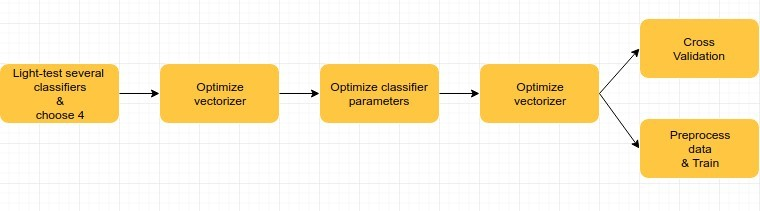
\includegraphics[width=13cm]{scikitWorkflow.jpg}
    \caption{Implementation workflow of sentiment analysis using Scikit module}%
    \label{fig:scikitWorkflow}%
\end{figure}

After manually testing and playing around with all sci-kit classifiers which are mostly used for analysis of textual data, I've decided to continue working with four of them - \textbf{Logistic Regression, Linear support vector machine and 2 Naive Bayes classifiers for multinomial models.} I had high expectations especially from Bernoulli NB as it should perform better on shorter texts. I've measured their accuracy on Sentiment140 as well as movie reviews dataset. Just out of pure curiosity I've tried to train the classifiers on movie reviews and test them on tweets contained in Sentiment140. Obviously, such approach is not correct but I wanted to see how much worse will the classifiers perform. All metrics can be seen in table \ref{table:scikitOnSentiment140}.

\paragraph{Vectorizer and its optimizations}
Goal of this step is to find best performing vectorizer for feature extraction.	Vectorization is a step when "words are turned into numbers". While words can be transformed into numbers, an entire document can be translated into a vector. Not only can a vector have more than one dimension, but with text data vectors are usually high-dimensional. This is because each dimension of your feature data will correspond to a word, and the language in the documents you are examining will have thousands of words.

The most common and simplest vectorizer approach is \textbf{bag of words}.	In this approach, union of all the words from all documents in the corpus is the dimension of the vector which is created. That means that 800 documents with 1000 words would result in 1000-dimensional vector where every unique word has its own index in that vector. Every document is processed with so called "one-hot" encoding where basically every word in the corpus is looked up in the document and zero/one is assigned accordingly. It results to every document being represented by zeros and ones. This approach has been used in my classifier built with NLT python module described in previous section. Bag of words approach is naïve in the sense that it does not distinguish the context of how a sentence or paragraph is structured. It pays attention to frequency of words but completely ignores things like position of the word in the sentence. The solution for this are N-grams. Using N-grams, vector is encoded for various combinations of words rather than just single words. This helps to preserve semantic meaning better but also causes the vector dimensionality increase. Bag of Words also can’t tell you whether or not words are unique, as the fact that a word is showing up repeatedly within a certain type of document can hint at its importance. Solution for this problem is to employ \textbf{Term Frequency-Inverse Document Frequency (TFIDF) Matrix} as a vectorization approach. That's also the vectorizer I have used for my classifier. TFIDF allows to place more emphasis on infrequent words by assigning a weight to each word instead of a binary value. The weight is determined through a combination of the word’s frequency in a document, and how rare the word is in the entire corpus.

Once I've decided which vectorizer class to use, there is also a question which parameters should I use it with. Sci-kit module offers “GridSearchCV” class which is a way how to conveniently find the best combination of all specified vectorizer parameter values. Altogether were tested and evaluated 92 vectorizers. Testing method and values examined can be seen in the following listing \ref{lst:vectorizerGridsearchcv}. 

\begin{lstlisting}[caption={Tuning of vectorizer using “GridSearchCV” class },label={lst:vectorizerGridsearchcv},language=Python]
    def tuneVectorizerParameters(corpus,labels):
    	pipeline = Pipeline([
        	('tfidf', TfidfVectorizer(stop_words='english')),
        	('clf', LinearSVC()),
    	])
    	parameters = {
        'tfidf__max_df': (0.75, 0.9),
        'tfidf__ngram_range': [(1, 1), (1, 2), (1, 3)],
        'tfidf__sublinear_tf': (True, False),
        'tfidf__stop_words':['english']
    }

    grid_search_tune = GridSearchCV(pipeline, parameters, cv=2, n_jobs=2, verbose=3)
    print("Searching best parameters combination:")
    grid_search_tune.fit(corpus, labels)

    print("Best parameters set:")
    print grid_search_tune.best_estimator_.steps
\end{lstlisting}

\paragraph{Classifier optimizations}
All classification algorithms have several parameters which can adjust and possibly improve their performance. Choosing the correct parameters for machine learning algorithms or so called “tuning” process is a field in itself and separate thesis could be written just about this. I have again used GridSearchCV class for this. For all algorithms, I have specified various values for several parameters, but even the performance for returned best parameter combination performed worse than the default parameters which are used in default constructor. Optimization of classifiers using “GridSearchCV” is briefly shown in the listing \ref{lst:classifierGridsearchcv}.

\begin{lstlisting}[caption={Tuning of classifiers using “GridSearchCV” class },label={lst:classifierGridsearchcv},language=Python]
    	scores = ['accuracy']
        # Set the parameters to combine
        SVC_parameters = [{'C': [1,10,100,1000],
                             'loss': ['hinge','squared_hinge'],
                             'multi_class': ['ovr','crammer_singer'],
                             'fit_intercept': [True,False]
                             }]
        MultiNB_parameters = [{'alpha': [1.0, 2.0, 5.0, 10.0],
                             'fit_prior': [True, False]
                             }]
        BernoulliNB_parameters = [{'alpha': [1.0, 2.0, 5.0, 10.0],
                                   'binarize': [0.0, 2.0, 5.0, 10.0],
                                 'fit_prior': [True, False]
                                 }]

        for score in scores:
            print("Tuning hyper-parameters for %s" % score)

            clf = GridSearchCV(LinearSVC(), SVC_parameters, cv=5,scoring='%s' % score)
            clf.fit(train_corpus_tf_idf, y_train)

            print("Best parameters set found:")
            print(clf.best_params_)
            print("Performance for all combinations:")
            means = clf.cv_results_['mean_test_score']
            stds = clf.cv_results_['std_test_score']
            for mean, std, params in zip(means, stds, clf.cv_results_['params']):
                print("%0.3f (+/-%0.03f) for %r"
                      % (mean, std * 2, params))

            print("Detailed classification report of model trained and evaluated on full dev/eval sets:")
            y_true, y_pred = y_test, clf.predict(test_corpus_tf_idf)
            print(classification_report(y_true, y_pred))
\end{lstlisting}    


\begin{table}[H]
\centering
\begin{tabular}{| p{3cm}|p{3cm}|p{5cm}|p{3cm}|}
 \hline
\textbf{ Training data }& \textbf{Test data} & \textbf{ Classifier }& \textbf{Accuracy}\\
 \hline
  \multirow{4}{*}{Sentiment140}   & \multirow{4}{*}{Sentiment140} & Linear SVM   & 0.785\\ 
    &  &  Multinomial Naive Bayes & 0.761\\ 
    &  &  Bernoulli Naive Bayes & 0.773\\  
    &  & Logistic Regression & 0.797\\ \hline 
  \multirow{4}{*}{Movie reviews}   & \multirow{4}{*}{Movie reviews} & Linear SVM   & 0.849\\ 
    &  &  Multinomial Naive Bayes & 0.807\\ 
    &  &  Bernoulli Naive Bayes & 0.792\\  
    &  & Logistic Regression & 0.823\\ \hline 
  \multirow{4}{*}{Movie reviews}   & \multirow{4}{*}{Sentiment140} & Linear SVM   & 0.560\\ 
    &  &  Multinomial Naive Bayes & 0.562\\ 
    &  &  Bernoulli Naive Bayes & 0.5\\  
    &  & Logistic Regression & 0.515\\ \hline 
\end{tabular}
\caption{Scikit classifiers accuracy on Sentiment140 dataset}
\label{table:scikitOnSentiment140}
\end{table}

As we can see, performance of these classifiers is much better than the previous one using Textblob. Despite 78\% accuracy might still sound pretty low, it's important to realize that Tweets are very short text pieces which often don't offer much sentiment input to work with. Therefore is 78\% quite promising performance for future work. For example, other paid services like MonkeyLearn \footnote{https://monkeylearn.com/} offer 81\% accuracy on Tweets sentiment classification.

Another thing I tried to increase the accuracy of the classifiers was preprocessing. First I have kept only words which contained only letters and then I have decided to get rid also of urls, punctuation, usernames and hastags. Accuracy metrics can be seen in table \ref{table:preprocesingAccuracy}. Training and testing data were from Sentiment140. Performance boost was smaller that expected but still, any improvement is better than none.

\begin{table}[H]
\centering
\begin{tabular}{|p{5cm}|p{5cm}|p{3cm}|}
 \hline
\textbf{Preprocessing type} & \textbf{ Classifier }& \textbf{Accuracy}\\
 \hline
 \multirow{4}{*}{\parbox{5cm}{\centering Just words with letters}} & Linear SVM   & 0.785\\ 
   &  Multinomial Naive Bayes & 0.76\\ 
   &  Bernoulli Naive Bayes & 0.772\\  
   & Logistic Regression & 0.796\\ \hline 
  \multirow{4}{*}{\parbox{5cm}{\centering Stripped URLs, punctuation, usernames, alphanumetric characters, hashtags}} & Linear SVM   & 0.786\\ 
   &  Multinomial Naive Bayes & 0.766\\ 
   &  Bernoulli Naive Bayes & 0.774\\  
   & Logistic Regression & 0.795\\ \hline 
\end{tabular}
\caption{Scikit classifiers accuracy on Sentiment140 dataset}
\label{table:preprocesingAccuracy}
\end{table}


\paragraph{Neutral Tweets}: At this point, after all the tuning, optimizing and cross-validation, I could finally run my analyzer on the testdata also provided by Sentiment140. Compared to the training data which contain just positive and negative tweets, test file contains also neutral ones. Obviously, this is a problem, since my classifiers are not familiar with the concept of neutral tweets. In current state, accuracy on a test set with neutral tweets is just 58.4\% whereas on the same test set with excluded neutral tweets, accuracy was more than 81\% - which is expected because it's basically the same set just with different tweets which has also been used	 during cross-validation. 

In general, third neutral class in sentiment analysis is still causing big problems. E.g Go, Huang and Bhayani \cite{go2009twitter2} considered any tweet without an emoticon to be part of the neutral class, which they themselves admitted to be a flawed approach. Kouloumpi at al. \cite{kouloumpis2011twitter} trained their classifier just on hashtags and emoticons and also had to build their own neutral training dataset.  Agarwal at al \cite{agarwal2011sentiment} annotated their own training dataset to contain neutral tweets and achieved very nice accuracy of 60\% which is much higher than the base line of 33\%. Although it is a nice result, they had training data which contained neutral data. Saif et al. \cite{saif2012semantic} as well as Go, Huang and Bhayani \cite{go2009twitter} in their second article that year just stated that identifying neutral tweets is part of their future work plan.  Afer realizing that doing a tree way analysis rather than just binary or qualitative (output is a score value) analysis is worth a separate thesis I have decided to train my classifier for only weighted qualitative output in interval from 0 to 1, where 1 is the most positive. Just out of curiosity, I've     defined confidence thresholds for positive and negative tweets. Everything which would be between these 2 threshold levels could be considered a neutral tweet. I manually tried several values and accuracy scores from these measuments are recorded in table \ref{table:negativeAccuracy}. I've achieved accuracy just 7\% above the baseline at most, so the lack of optimization for neutral tweets classification is obvious.\\
\\
\begin{table}
\centering
\begin{tabular}{|p{4cm}|p{4cm}|p{3cm}|}
 \hline
\textbf{ Negative threshold }& \textbf{Positive threshold} & \textbf{Accuracy}\\
 \hline
 0.1 & 0.9 & 0.357\\ \hline
 0.2 & 0.8 & 0.385\\ \hline
 0.3 & 0.7 & 0.393\\ \hline 
 0.4 & 0.6 & 0.401\\ \hline 
\end{tabular}
\caption{Sci-kit accuracy with various handling of neutral tweets}
\label{table:negativeAccuracy}
\end{table}

\textbf{Abstracting several classifiers under one custom classifier}:
I later came up with an idea of abstracting all classification algorithms all under one custom classifier. My custom classifier is able to be trained in 3 modes - as a binary classifier, multiclass classifier or a classifier outputting a float confidence score of text being positive.
This approach has of course both, advantages and disadvantages as well. Advantage for sure is that possibility of False positives or False Negatives is much lower as this requires 3 incorrect classifications to instead of 1. Trade-off for this is that the confidence score of being positive is in general lower because the possibility of at least one of 3 algorithms being wrong is (obviously) higher than if there is only one single classifier.\\

All performance matrices of the final classifier for various datasets are displayed in figure \ref{fig:finalClassifierPerformanceBarChart}.
\\

\begin{figure}%
    \centering
	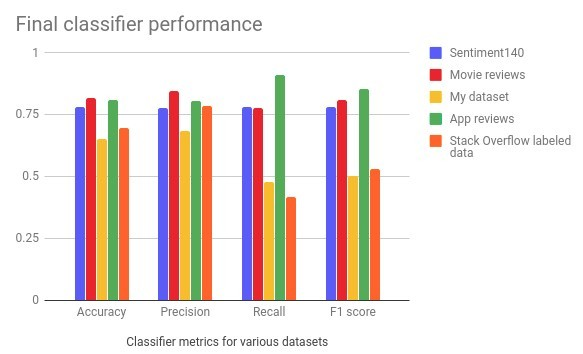
\includegraphics[width=14cm]{finalClassifierPerformanceBarChart.jpg}
    \caption{Final classifier performance for several datasets}%
    \label{fig:finalClassifierPerformanceBarChart}%
\end{figure}

It's clear that the best results are achieved with movie or app reviews because these texts offer more features to draw the sentiment from because they are longer texts. We can also see that training datasets built from shorter texts (My twitter dataset or SO labeled dataset created and used in Bin Li's paper ) have worse performance, especially recall. With my own dataset, its size might be causing this as it contains only 84 labeled entries. I concluded that using Sentiment140 as a definitive training dataset is a good choice as its performance is just sligthly worse compared to reviews but it's still authentic Twitter data which I'm going to analyze the most.

\section{Data to analyze}
I found Twitter data very suitable for sentiment analysis and therefore decided to analyze only tweets and use SO and Reddit later in chapter \ref{chap:pairingBugs}  about recognizing bugs in discussions.

Using the steps described in section \ref{ssec:GettingData}, I've downloaded tweets with following time conditions/patterns:
\begin{itemize}
\item between two immediate releases
\item on release dates
\item weekly
\end{itemize}



\section{Results}
\subsection{Immediate sentiment change with releases}
First and the most simple analysis was to compare sentiment of tweets collected 3 days prior and post-release. Results are shown in table \ref{table:BeforeAfterReleaseSentiment}.

\begin{table}[H]
\centering
\begin{tabular}{ |p{3cm}|p{3cm}|p{3cm}|}
 \hline
\textbf{Project }& \textbf{Before}& \textbf{After}\\
 \hline
 NodeJS   & 0.707 & 0.709\\ \hline
 EmberJS   & 0.719 & 0.719\\ \hline
 VueJS   & 0.694 & 0.708\\ \hline 
 Symfony & 0.73 & 0.729\\ \hline   
 AngularJS   & 0.718 & 0.719\\ \hline
 CakePhp & 0.71 & 0.702\\ \hline 
 Bower   & 0.634 & 0.638\\ \hline 
 Laravel & 0.683 & 0.696\\ \hline
 Gulp & 0.608 & 0.573\\ \hline
 Yii & 0.643 & 0.606\\ \hline
 Bootstrap & 0.713 & 0.693\\ \hline
\end{tabular}
\caption{Average sentiment of tweets 3 days before and after releases}
\label{table:BeforeAfterReleaseSentiment}
\end{table}

From the data shown in table is visible, that there is no big sentiment shift caused by releases on the small time frame. The biggest noticable pattern (nicely displayed in figure \ref{fig:sentimentChangeBeforeAfter}) is 4\% decrease in sentiment of seldom releasing projects. In groups which release often or normally, sentiment change was very small. A clear pattern to notice in figures \ref{fig:weeklyAverageBarchart} and \ref{fig:sentimentChangeBeforeAfter} is, that more often projects release, better the sentiment gets.

\begin{figure}%
    \centering
	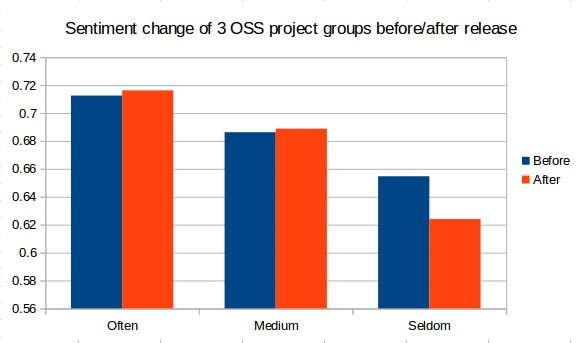
\includegraphics[width=10cm]{sentimentChangeBeforeAfter.jpg}
    \caption{Change in sentiment for all 3 OSS groups before/after release}%
    \label{fig:sentimentChangeBeforeAfter}%
\end{figure}

\subsection{Results for weekly collected data}
First and the most simple analysis was to compare sentiment of tweets collected with period one week. I have also added the sentiment of some projects' Reddit discussions (keep in mind that classifier is trained on tweets, so this is not the best approach). Results can be seen in Table \ref{table:weeklyAverageTable} and Figure \ref{fig:weeklyAverageBarchart}.

\begin{table}[H]
\centering
\begin{tabular}{ |p{2cm}|p{5.5cm}|p{5.5cm}|}
 \hline
\textbf{Project }& \textbf{Twitter average sentiment} & \textbf{Reddit average sentiment}\\
 \hline
 NodeJS   & 0.697   & 0.633 \\ \hline
 EmberJS   & 0.709   & 0.69\\ \hline
 VueJS   & 0.715   & 0.60\\ \hline 
 Symfony & 0.727   & *\\ \hline   
 AngularJS   & 0.727   & 0.618\\ \hline
 CakePhp & 0.703  & * \\ \hline 
 Bower   & 0.641   & No subreddit\\ \hline 
 Laravel & 0.701   & *\\ \hline
 Gulp & 0.578   & No subreddit\\ \hline
 Yii & 0.658  & * \\ \hline
 Bootstrap & 0.713  & 0.635\\ \hline
 \multicolumn{3}{l}{* Reddit changed its API and submissions endpoint is not supported anymore}
\end{tabular}
\caption{Average sentiment of tweets collected weekly}
\label{table:weeklyAverageTable}
\end{table}


\begin{figure}[H]%
    \centering
	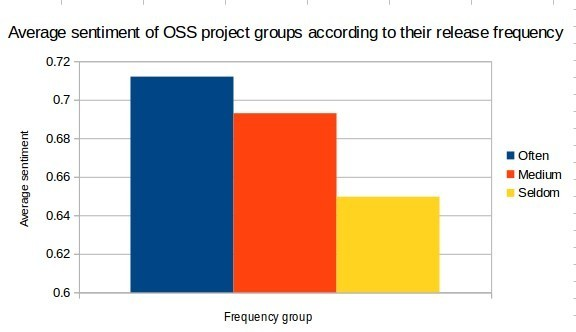
\includegraphics[width=11cm]{weeklyAverageBarchart.jpg}
    \caption{Average sentiment of OSS project groups according to their release frequency}%
    \label{fig:weeklyAverageBarchart}%
\end{figure}

In both of previous analysis, I have used the simplest aggregation operation which is average. Replacing this one with median, modus or some more advanced aggregations could potentially yield different results but because each group is represented just by 3 or 4 OSS projects, losing any data would actually be a significant part of the overall analysed dataset. Using more projects could be potentially a part of future work.

\subsection{Cross-correlation between releases and sentiment change} \label{ssec:crossCorrelation}
When working with time series, we often want to determine whether one series causes changes in another. To find this relationship, measuring a cross-correlation and finding a lag is one way how to do it. Lag represents when change in one data series transfers to the other several periods later. 

To ensure a cross-correlation calculation makes sense, first I have to determine, whether are the data stationary. A stationary time series is one whose properties do not depend on the time at which the series is observed\cite{hyndman5forecast}. More precisely, if y\textsubscript{t} is a stationary time series, then for all \textit{s}, the distribution of \textit{(y\textsubscript{t},…,y\textsubscript{t+s})} does not depend on \textit{t}.

To determine whether my data are stationary, I've used the Dickey-Fuller test method of tseries package in R. Results can be seen in the table \ref{table:stationarity_table_sentiment} and \ref{table:stationarity_table_release_count} 

\begin{table}[H]
\centering
\begin{tabular}{ |p{3cm}||p{3cm}|p{3cm}|  }
 \hline
 \multicolumn{3}{|c|}{Stationarity test of web frameworks sentiment data} \\
 \hline
 Framework & Dickey-Fuller & p-value\\
 \hline
 NodeJS   & -2.6775    &0.2964\\ \hline
 AngularJS &   -3.883  & 0.0199\\ \hline
 EmberJS & -4.0783 & 0.0199\\ \hline
 VueJS    &-3.438 & 0.0646\\ \hline
 CakePHP&   -3.480  & 0.04847\\ \hline
 Laravel& -2.57  & 0.3431\\ \hline
 Symfony& -4.3979  & 0.01\\ \hline
\end{tabular}
\caption{Stationarity test of sentiment}
\label{table:stationarity_table_sentiment}
\end{table}

\begin{table}[H]
\centering
\begin{tabular}{ |p{3cm}||p{3cm}|p{3cm}|  }
 \hline
 \multicolumn{3}{|c|}{Stationarity test of web frameworks release count} \\
 \hline
 Framework & Dickey-Fuller & p-value\\
 \hline
 NodeJS   & -2.896    &0.205\\ \hline
 AngularJS &   -2.547  & 0.353\\ \hline
 EmberJS & -3.297 & 0.0802\\ \hline
 VueJS    &-2.158 & 0.511\\ \hline
 CakePHP&   -3.224  & 0.08915\\ \hline
 Laravel& -2.368  & 0.425\\ \hline
 Symfony& -2.218  & 0.488\\ \hline
\end{tabular}
\caption{Stationarity test of release counts}
\label{table:stationarity_table_release_count}
\end{table}

As we can see, p-values are always higher than 0.05 what indicates non-stationarity of the data, therefore I can't calculate the cross-correlation on them in this state. To transform non-stationary data into stationary, 2 approaches can be used. These are differencing and transforming.  I've taken data series and differenced the values in listing \ref{lst:differencing}. I've executed both, seasonal differencing and stationary differencing although seasonal probably was not needed because the data should not be dependant on the season.

\begin{lstlisting}[caption={Used differencing method in R},label={lst:differencing},language=R]
Differencing <- function(x,y)
{
 framework_x_seasdiff <- diff(x,differences=1)  # seasonal differencing
 framework_x_Stationary <- diff(framework_x_seasdiff, differences= 1)
 framework_y_seasdiff <- diff(y, differences=1)
 framework_y_Stationary <- diff(framework_y_seasdiff, differences= 1)
 return(list(framework_x_Stationary,framework_y_Stationary))
}
\end{lstlisting}
New differenced values do appear to be stationary in mean and variance, as the level and the variance of the series stays roughly constant over time. Sentiment for NodeJS before and after differencing can be seen in Figure \ref{fig:NodeJS_Sentiment_before_after}

\begin{figure}[H]%
    \centering
    \subfloat[Before differencing]{{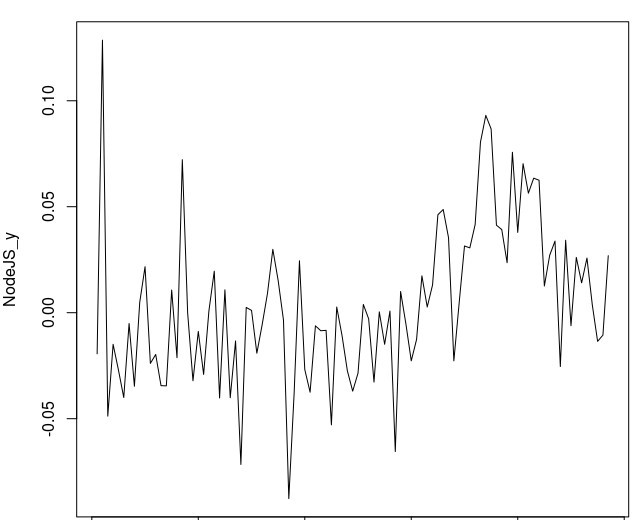
\includegraphics[width=6cm]{NodeJS_before.jpg} }}%
    \qquad
    \subfloat[After differencing]{{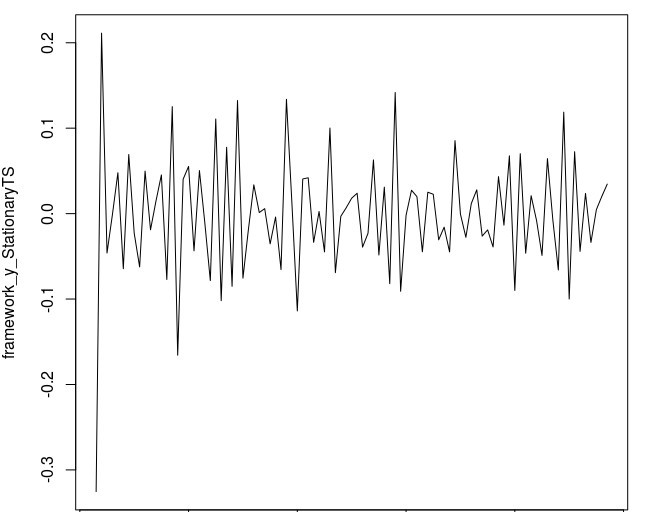
\includegraphics[width=6cm]{NodeJS_after.jpg} }}%
    \caption{NodeJS monthly sentiment values}%
    \label{fig:NodeJS_Sentiment_before_after}%
\end{figure}

Same procedure needed to be done with the "number of releases per month" data and afterwards. Then, cross-correlation could be executed. For this task I've used ccf method in R which implements Pearson's correlation calculation method. Results for all 7 OSS projects can be seen in Figure \ref{fig:highestCorrelationsPlotReleases}

\begin{figure}[H]%
    \centering
	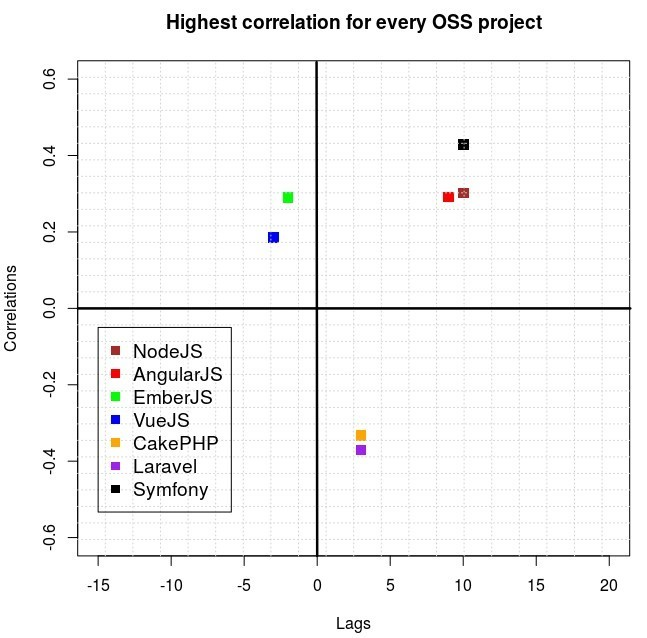
\includegraphics[width=8cm]{highestCorrelationsPlotReleases.jpg}
    \caption{Highest correlations for every OSS project}%
    \label{fig:highestCorrelationsPlotReleases}%
\end{figure}

\paragraph{Results interpretation:}

As we can there is no general pattern. Maximal project correlations happen to occupy 3 of 4 possible quadrants. Each quadrant represents a different relationship between number of releases and sentiment change.

\begin{itemize}
  \item \textbf{I. Quadrant}(Positive correlation + positive lag) - Increase of release count increases a sentiment
  \item \textbf{II. Quadrant}(Positive correlation + negative lag) - Increase of sentiment increases a release count
  \item \textbf{III. Quadrant}(Negative correlation + positive lag) - Increase of release count decreases a sentiment
  \item \textbf{IV. Quadrant}(Negative correlation + Negative lag) - Increase of sentiment decreases a release count
\end{itemize}

Also, in Figure \ref{fig:highestCorrelationsPlotReleases_nonStat} are the results without making the data series stationary. It's obvious that making the data stationary has a big impact on the results.

\begin{figure}[H]%
    \centering
	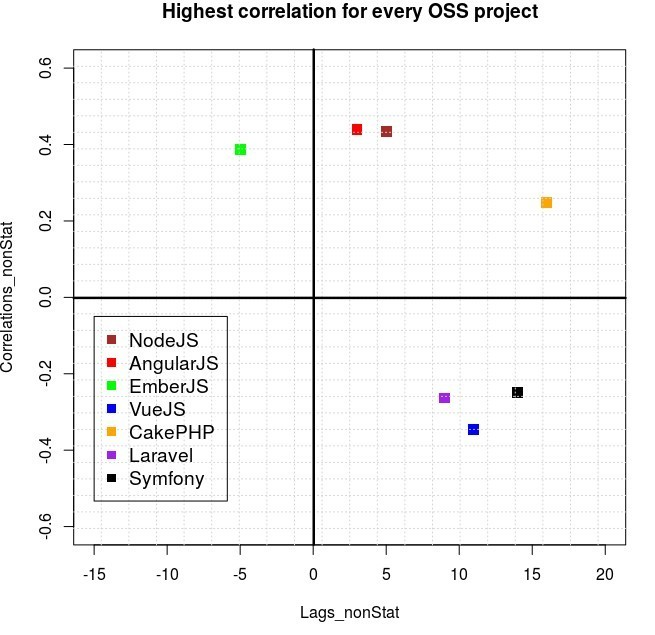
\includegraphics[width=8cm]{highestCorrelationsPlotReleases_nonStat.jpg}
    \caption{Highest correlations for every OSS project (non-stationary)}%
    \label{fig:highestCorrelationsPlotReleases_nonStat}%
\end{figure}

\subsection{Commits count within releases} \label{ssec:crossCorrelationCommits}
Initially, I thought that to modify project to take into account a size of the release (amount of commits) will be pretty straightforward task. It actually was straightforward, but as always I've encountered several unexpected problems on the way. \\
I intended to extend my previously used method from Section \ref{ssec:gitReleaseDatesMining} which uses Git API tags endpoint to get the release dates. Unfortunately I wasn't able to find number of commits in the returned objects. JSON object returned from API has following structure:
\begin{lstlisting}
  {
    "url": X,
    "assets_url": X,
    "upload_url": X,
    "html_url": X,
    "id": X,
    "tag_name": X,
    "target_commitish":X,
    "name": X,
    "draft": X,
    "author":{},
    "prerelease": X,
    "created_at": X,
    "published_at": X,
    "assets":[],
    "tarball_url": X,
    "zipball_url":X, 
    }
\end{lstlisting}
I have done some extra searching but did not want to spend extra time so I decided to go the way I knew will work. Instead of using API to get the commit counts, I crawled GitHub UI page of each release and extracted information directly from page source code. Each release details page provides information how many commits behind the current HEAD the commit is. The difference in this number between two following releases represents count of new commits for a release. Results of simple tabular substraction with spreadsheet formula needed to be manually corrected because projects often release several branches parallel and therefore substraction from the previous release was not always the correct one.\\
\\
Eventually, I got correct number of commits for every release and could execute the same cross-correlation analysis described in the previous chapter, but this time instead of releases count, I have explored relationship between sentiment and commits count. One possible flaw in the commit count data are the pre-releases. I treated them as normal releases because they do offer new features but those very same commits are then counted in the official releases later on.\\
\\
After getting the data ready I performed a stationarity test for commit counts. Sentiment values are the same as before with count of releases. Table \ref{table:stationarity_table_commits} shows the results.

\begin{table}[H]
\centering
\begin{tabular}{ |p{3cm}||p{3cm}|p{3cm}|  }
 \hline
 \multicolumn{3}{|c|}{Stationarity test of web frameworks commit counts} \\
 \hline
 Framework & Dickey-Fuller & p-value\\
 \hline
 NodeJS   & -7.0239    &0.01\\ \hline
 AngularJS &   -2.547  & 0.3531\\ \hline
 EmberJS & -3.2764 & 0.0831\\ \hline
 VueJS    &-2.9748 & 0.1886\\ \hline
 CakePHP&   -3.655  & 0.03283\\ \hline
 Laravel& -2.919  & 0.2084\\ \hline
 Symfony& -4.8461  & 0.01\\ \hline
\end{tabular}
\caption{Stationarity test of commit counts}
\label{table:stationarity_table_commits}
\end{table}

I see that there are again several data series (AngularJS, EmberJS, VueJS, Laravel + NodeJS because of unstationarity of sentiment data) which are not stationary so exactly as before with release counts, I had to transform the data. After that, Pearson's cross correlation was calculated. Results for all 7 OSS projects can be seen in Figure \ref{fig:highestCorrelationsPlot}

\begin{figure}[H]%
    \centering
	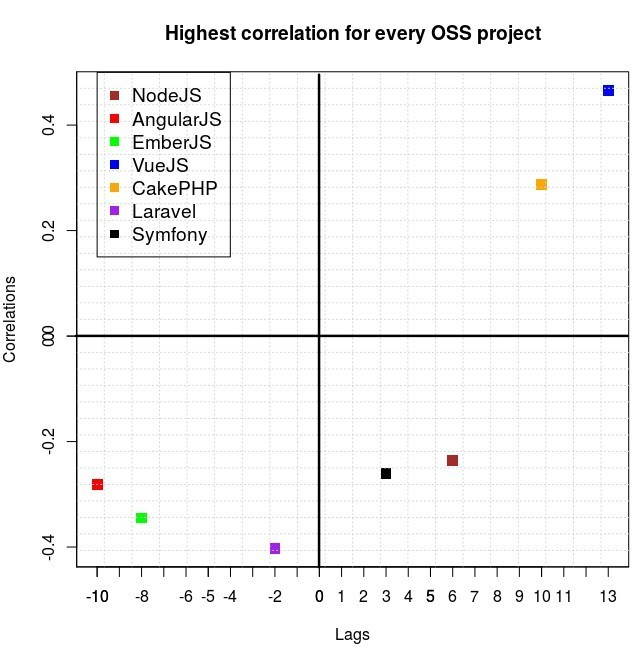
\includegraphics[width=8cm]{highestCorrelationsPlot.jpg}
    \caption{Highest correlations for every OSS project}%
    \label{fig:highestCorrelationsPlot}%
\end{figure}

If I would skip the step of making the data stationary, results would again look completely different \ref{fig:highestCorrelationsPlot_nonStat}.

\begin{figure}[H]%
    \centering
	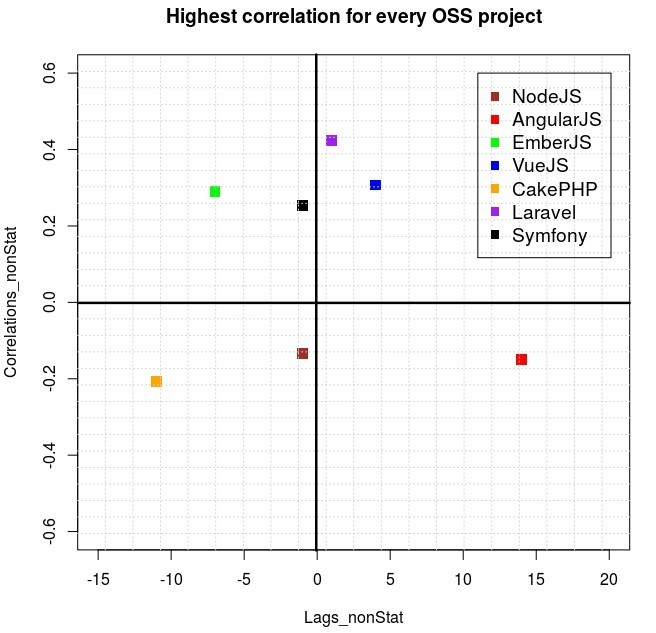
\includegraphics[width=8cm]{highestCorrelationsPlot_nonStat.jpg}
    \caption{Highest correlations for every OSS project (non-stationary)}%
    \label{fig:highestCorrelationsPlot_nonStat}%
\end{figure} 
